%-----------------------------------------------------------------------------
%
%               Template for sigplanconf LaTeX Class
%
% Name:         sigplanconf-template.tex
%
% Purpose:      A template for sigplanconf.cls, which is a LaTeX 2e class
%               file for SIGPLAN conference proceedings.
%
% Guide:        Refer to "Author's Guide to the ACM SIGPLAN Class,"
%               sigplanconf-guide.pdf
%
% Author:       Paul C. Anagnostopoulos
%               Windfall Software
%               978 371-2316
%               paul@windfall.com
%
% Created:      15 February 2005 
%
%-----------------------------------------------------------------------------


\documentclass[10pt,draft]{sigplanconf}

% The following \documentclass options may be useful:

% preprint      Remove this option only once the paper is in final form.
% 10pt          To set in 10-point type instead of 9-point.
% 11pt          To set in 11-point type instead of 9-point.
% authoryear    To obtain author/year citation style instead of numeric.

\usepackage{graphicx}
\usepackage{amsmath}
\usepackage[obeyDraft]{todonotes}
\usepackage{listings}
\usepackage{xspace}
\usepackage{verbatim}
\usepackage{booktabs}
\usepackage{url}
\usepackage{siunitx}
\usepackage{relsize}

\setkeys{Gin}{draft=false} % Show images in draft mode
\graphicspath{ {graphics/} }

\begin{document}
\presetkeys{todonotes}{inline}{}

\special{papersize=8.5in,11in}
\setlength{\pdfpageheight}{\paperheight}
\setlength{\pdfpagewidth}{\paperwidth}

\conferenceinfo{DLS '15}{October 25--30, 2015, Pittsburgh, PA, USA} 
\copyrightyear{2025} 
\copyrightdata{978-1-nnnn-nnnn-n/yy/mm} 
\doi{nnnnnnn.nnnnnnn}

% Uncomment one of the following two, if you are not going for the 
% traditional copyright transfer agreement.

\exclusivelicense                % ACM gets exclusive license to publish, 
                                  % you retain copyright

%\permissiontopublish             % ACM gets nonexclusive license to publish
                                  % (paid open-access papers, 
                                  % short abstracts)

\titlebanner{banner above paper title}        % These are ignored unless
\preprintfooter{short description of paper}   % 'preprint' option specified.

\title{Language Independent Storage Strategies}
%\subtitle{Subtitle Text, if any}

\authorinfo{Anton~Gulenko}
		   {Technische Universit\"at Berlin}
           {anton.gulenko@tu-berlin.de}
\authorinfo{Tobias~Pape\and{}Tim~Felgentreff\and{}Robert~Hirschfeld}
           {Hasso Plattner Institute, University of Potsdam}
           {\{firstname.lastname\}@hpi.uni-potsdam.de}
\authorinfo{Carl~Friedrich~Bolz}
           {King's College, London}
           {cfbolz@gmx.de}

% ============== Notes ==============

% ===== Approach, Framework Description
% deutliche Herausstellung des eigenen Beitrags
% Wie kam es zur Auswahl der aktuellen Strategien? (Anforderungen, Heuristiken, ...)
% Infrastruktur (Framework?) zur Verwaltung der Strategien?
% Lebenszyklus von Strategien usw.
% Können Objekte/Collections ihre Storage-Strategies zur Laufzeit anpassen? (Wurde im Vortrag nicht deutlich...)

% ===== Figures
% Legenden zu Abbildungen (darauf passen wir dann im Paper auf)
% Zustandsübergänge mit 0.0%

% ===== Evaluation
% Benchmarks evtl. auch relativ zu Interpreter- und Cog-VMs (Praktikabilität, ...)
% Szenario für Benchmark/Messung genauer beschreiben (Umfang, Zeitdauer, ...) und wiederholen

% ===== Future Work
% Welche Strategien wäre noch denkbar? -> Umfang, Vollständigkeit, Praktikabilität, ...


\maketitle

\begin{abstract}
This is the text of the abstract.
\end{abstract}

\category{CR-number}{subcategory}{third-level}

% general terms are not compulsory anymore, 
% you may leave them out
\terms
term1, term2

\keywords
keyword1, keyword2

\section{Introduction}

Virtual Machines for dynamic programming languages depend on runtime optimizations to achieve appropriate performance.
One optimization that has been shown to work great in the Python VM PyPy is storage strategies.

Storage strategies try to optimize collection data types by transparently inlining their elements data, instead of holding references to actual objects.
Object allocations can be avoided because memory for the objects is already reserved in the collection itself.
In contrast to virtual objects, this optimization is applicable to any objects, not only those that don't escape the loop that is being optimized by the JIT.
Still, certain conditions have to be met in order to apply storage strategies.
These conditions are hard to detect even with the information available to a tracing JIT.
Therefore storage strategies have been implemented for PyPy \cite{strategies}, an RPython based Python interpreter, but are not automatically provided by the RPython toolchain.

\citeauthor{strategies} have shown that storage strategies are beneficial for the Python programming language\cite{strategies}.
Since Python offers one generic list data type, optimizing it can have a big impact on program performance.
We argue that \citeauthor{strategies}'s approach can be generalized and applied to other programming languages like Smalltalk or Ruby, which have rich collection standard libraries.
In this paper we investigate how we can make the storage strategy approach generic and gain its performance benefits in other contexts than the Python programming language.

We show that storage strategies is indeed beneficial for many dynamic languages.
We present a generic, language-independent implementation of the storage strategies optimization which can be reused in any VM implemented with the RPython toolchain.
We evaluate our implementation in two directions: generality and performance.



%\todo{The initial paper on strategies concluded with the "suspicion" that storage
%strategies are applicable to "virtually any" dynamic language, but that that'll
%have to be determined, and that possibly other "exotic" strategies may be needed,
%depending on the language semantics. We set out to support that suspicion, and
%to provide a generic framework to make use of strategies in a variety of dynamic
%languages easy}

%\todo{Contributions ... need to think about those, below just suggestions}
%\begin{itemize}
%\item An application of strategies to object storage in RSqueak
%\item A generic framework to add strategies to other PyPy-based languages
%\item An evaluation of the strategies approach for a wider range of languages
%\item Two-fold evaluation of presented approach: performance and generality
%\end{itemize}

\section{Background: Storage Strategies in PyPy}



\subsection{Static Objects}
\label{cha:staticObjects}

\todo{Removed this section?}

The most important optimization implemented by RPythons tracing JIT is an aggressive escape analysis \cite{escapeAnalysis}.
The escape analysis is conducted using a form of partial evaluation \cite{allocRemJIT}.
In short, it works by traversing the original trace, replacing object allocations with \emph{static objects}, and turning a static object back to a normal allocation when it is observed to escape the trace.
A static object is allocated directly on the stack, effectively avoiding the heap allocation.
This optimization is safe because the optimizer can prove that static objects don't affect the program state after the program exits the loop.

For an example, consider the \lstinline{SmallInteger} objects created inside the loop in listing \ref{lst:TraceExample1} on page \pageref{lst:TraceExample1}.
These \lstinline{SmallInteger} objects are not escaping the loop, because the only reference to each object is deleted at the end of each iteration.
Only the object allocated in the very last iteration persists after the loop ends.
Thus, all intermediate \lstinline{SmallInteger} instances don't need to be allocated; they are treated as static objects.
Their content is maintained on the stack instead of the heap, potentially even optimized into machine registers.

The drawback of static objects is a rather complex deoptimization.
As mentioned above, an optimized JIT trace must be left when a guard check, inserted to ensure correctness of the code, fails.
In such a case the escape analysis performed as basis for the static object optimization does not hold anymore.
Static objects allocated in the last loop iteration have to be allocated on the heap, and their contents have to be copied from the stack to the newly allocated objects.
To do this, the JIT has to maintain information about the stack layout while executing an optimized trace; using a stack map, the stack can be walked in order to create non-static versions of the objects.

Since RPythons meta tracing JIT creates traces of VM operations, not only language level objects can be turned into static objects, but also VM level objects.
Just like other optimizations in the RPython toolchain, this leads to cleaner code; short living objects can substantially increase the expressiveness of VM code.


\subsection{Storage Strategies}
\label{cha:storageStrategies}

Usually, collections in dynamic languages are represented by allocating an array and filling it with pointers that point to the actual elements of the collection.
This is because in a dynamic language, or even any language with polymorphism, objects of different types can be added to the same collection.
Using an array of pointers is the generic way to represent such a dynamic collection.
However, it also introduces an indirection between the collection and the actual elements.
To access any value from the collection, the VM must first fetch the pointer address and dereference it, before fetching the actual value.
This additional memory access is a big overhead compared to a C array of pure integer values, that a program can traverse in full speed.

Another allocation removal technique called storage strategies, or strategies for short, can optimize dynamic collections \cite{strategies}.
Storage strategies are implemented on VM level and are based on the idea that the VM has multiple possible ways of representing every collection internally.
Based on the user program and the operations performed on a collection, the VM can switch between multiple strategies and choose the most efficient one.
To do so, the collection contains a reference to the currently used strategy object, and all important operations performed on the collection are delegated to that object.
Ideally the strategy will not be switched very often, so the second important idea behind storage strategies is that user programs often utilize collections in a predictable way.

For example, collections are often used in a homogeneous way.
If the first few elements appended to a Python list are integers, then it is likely that the user program will keep storing only integer values in that list.
This is enough information to optimize the list.
In this case, the VM could allocate an array for integer values and store the values directly, without allocating box objects to represent these integers.
Figure \ref{fig:IntegerStorage} illustrates this example by showing two possible representations for the same collection: the collection on the left side contains boxed integer objects, while the collection on the right side contains pure integer values.

\begin{figure}[ht]
\centering
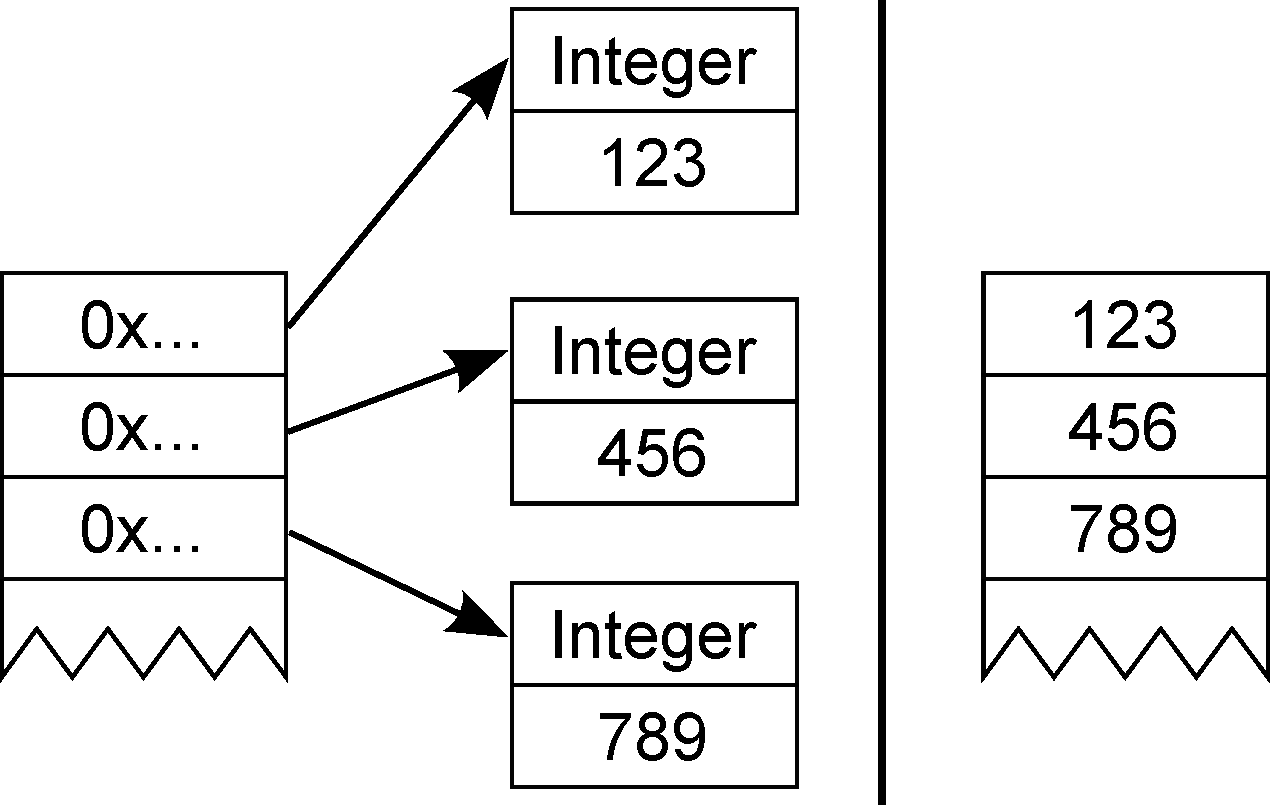
\includegraphics[width=0.4\textwidth]{strategies_intStorage}
\caption{Example for a storage strategy}
\label{fig:IntegerStorage}
\small
Left side: generic collection holding only boxed integer objects.\\
Right size: Optimized collection, resulting in less object allocations and memory usage.
\end{figure}

In order to optimize the internal representation of a collection, the VM must make assumptions about the usage pattern of that collection.
It cannot wait until a collection has been used for a while before optimizing it, otherwise it might end up not optimizing short living or small collections.
Optimizing short living collections can be very important, for example when they are allocated frequently in a tight loop.
In order to optimize as many collections as possible, the VM must predict the usage pattern based on the very first operations performed on a collection.

Making predictions about usage patterns is hard and the success can vary depending on the situation.
Therefore, the VM should make assumptions based on meaningful heuristics, which can be obtained by examining existing systems and deriving typical usage patterns.
But even with these preconditions there will be cases where the VMs assumptions turn out to be wrong.
In such cases, the VM must uphold the semantics of the programming language and perform a \emph{deoptimization}.
Most of the time this means allocating a new, more general collection and copying all elements from the old collection into the new one.
Figure \ref{fig:Deoptimization} shows an example of this procedure.
The storage on the left is optimized to hold integer values, but the user program wants to add a float value to the list.
The VM has to allocate a new, more general storage array which is able to hold generic objects.
In this case, the deoptimization could have been avoided if the VM had implemented a storage strategy to hold both integer and float values.
The deoptimization procedure must be tuned for highest performance, and should take place as rarely as possible.

\begin{figure}[ht]
\centering
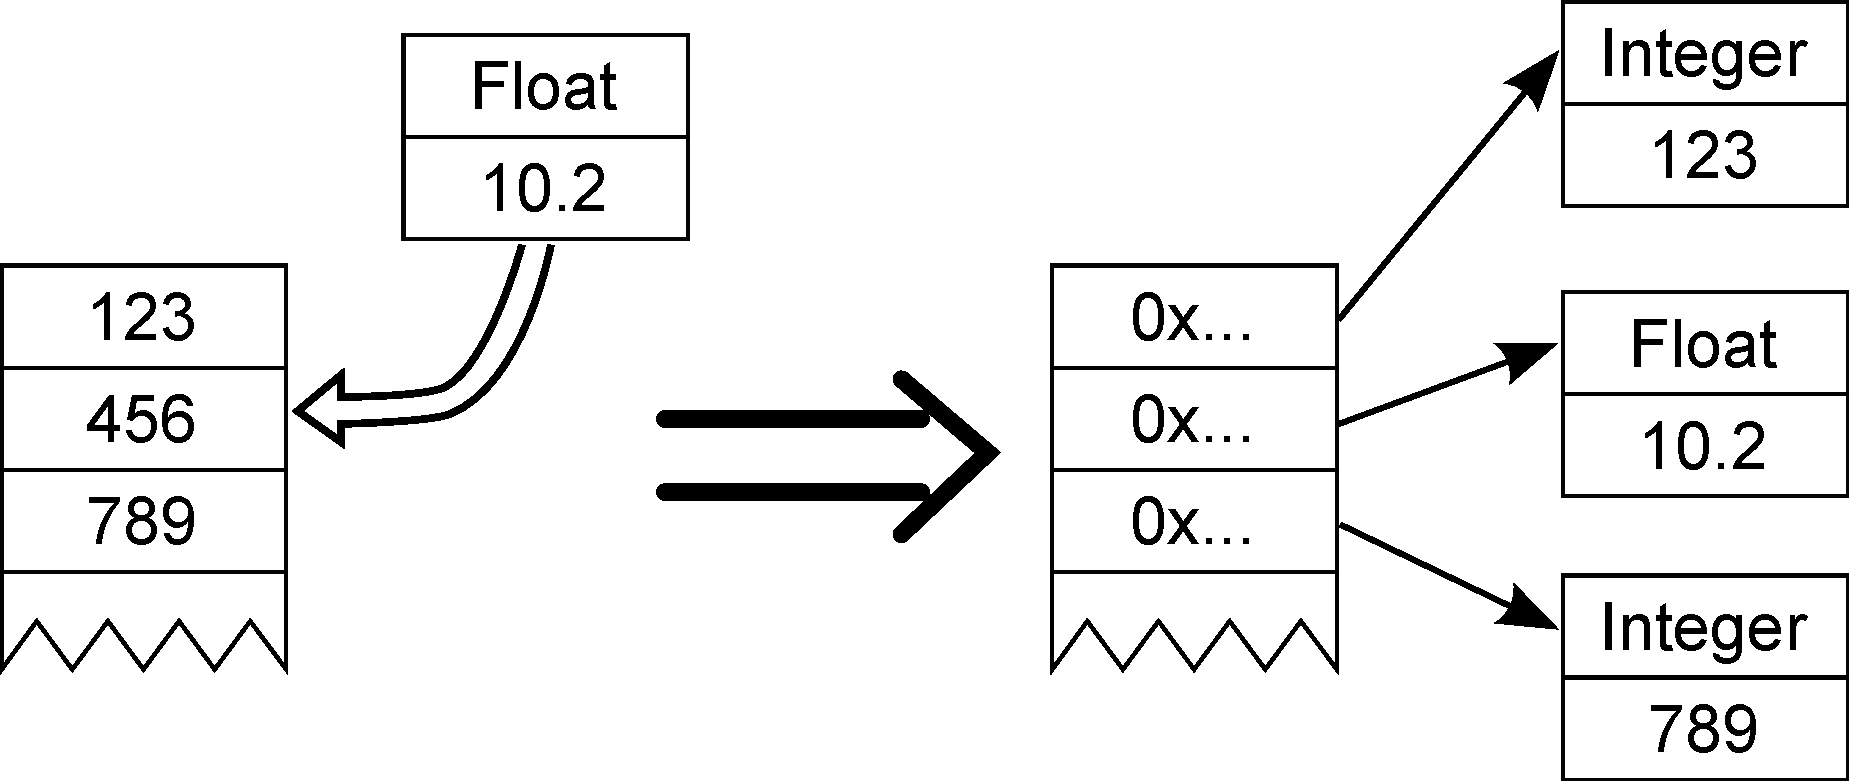
\includegraphics[width=0.4\textwidth]{strategies_deoptimization}
\caption{Deoptimization of an optimized integer collection}
\label{fig:Deoptimization}
\small
A general storage array has to be created, and Integer objects have to be allocated.
\end{figure}

\subsubsection{Homogeneous Collections}

As indicated by the examples in the previous section, the most important optimization target of storage strategies are homogeneous collections.
A collection is homogeneous when it only contains elements of a single type.
Since the size of the datatype is known, the VM can allocate an array big enough to hold the data of many such objects in consecutive memory.
The benefit of this optimization is two-fold: the VM can save the memory for the objects, and accessing the objects becomes faster due to the missing indirection between collection and elements.

This optimization is not limited to numeric datatypes like integers.
Even objects with multiple fields can be represented that way, as illustrated in figure \ref{fig:MultipleInlinedFields}.
The fields of each objects just have to be placed in memory in sequence.
Accessing any field in any object can happen without additional memory access, simply based on constant-time pointer arithmetics.

\begin{figure}[ht]
\centering
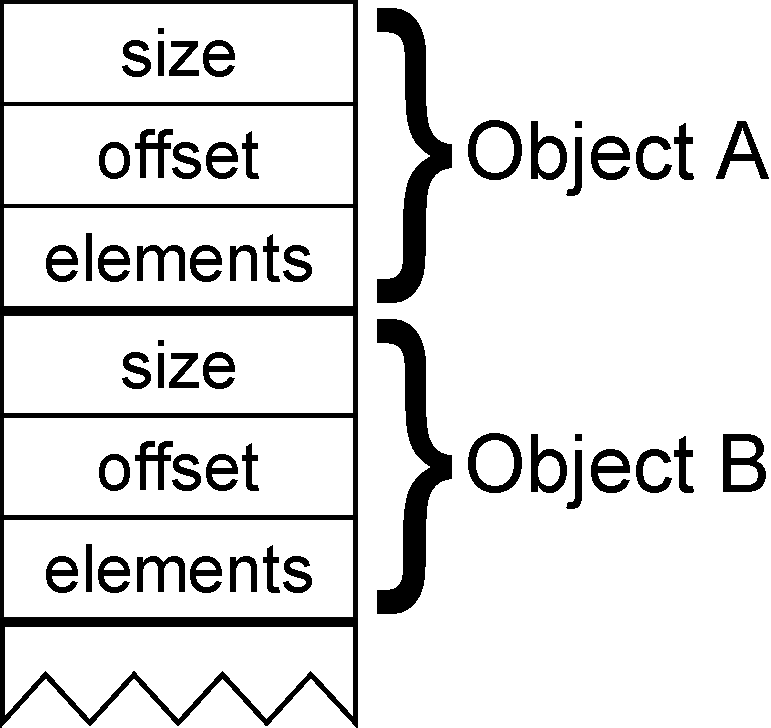
\includegraphics[width=0.27\textwidth]{strategies_multipleFields}
\caption{Inlining storage for composite objects with 3 fields}
\label{fig:MultipleInlinedFields}
\end{figure}

\section{Language Independent Storage Strategies}

%\subsection{The rstrategies Framework}
%\todo{Framework description}

%\subsection{Storage Strategies for Objects}
%\todo{RSqueak Implementation}
%\todo{which strategies are most important? why?}

%\subsubsection{Single Value Strategies}
%\todo{Nil}

%\subsubsection{Single Type Strategies}
%\todo{Int, Float}

%\subsubsection{Mixed Type Strategies}
%\todo{NilAndInt, NilAndFloat}

%\subsection{Supporting Exotic Objects}
%\todo{ContextParts, Classes, MethodDicts}


In this chapter we present the design of our library for storage strategies called rstrategies.
First we introduce the principles this library design is based on, then we describe different parts of the library and how a VM developer can utilize the library to create specific collection implementations.

In order to be reusable in the context of different programming languages, rstrategies must expose its functionality in a very flexible way.
We use the concept of mixins \cite{brachaMixins, mixins} to provide the required level of flexibility while allowing the VM to extend the provided functionality when needed.

In the context of RPython, any regular class can be used as a mixin.
The programmer must simply include a \lstinline{import_from_mixin(MixinClass)} clause into the body of the instantiating class.
All attributes and methods will then be copied over from \lstinline{MixinClass} to the target class, including all inherited methods.
A mixin is not intended to be used on its own.
It can require other mixins and fields or methods provided by the instantiating class itself.
This way the code inside a mixin can be written in an abstract way to promote modularity.

rstrategies supports two types of collections: variable sized and fixed sized lists.
These two abstract types of collections cover the needs of primitive collections for most programming languages.
The reasons behind this design decision are further explained in section \ref{sec:discussion}.

The rstrategies library provides a hierarchy of mixins that can be combined into actual collection classes.
If required, parts of the provided functionality can instead be implemented in the VM specific collection classes.
Any mixin class can also be extended in the VM specific code before being used.
There is one main mixin hierarchy that provides the largest part of the functionality.
At the top of this hierarchy is the class \lstinline{AbstractStrategy}.

\lstinline{AbstractStrategy} defines the interface implemented in its specific subclasses, in addition to a few internal methods.
The following methods are used to interact with the various storage strategy implementations:
\begin{description}
\item[store(index, item)]{Stores the given \lstinline{item} at the given \lstinline{index} in the collection. 
The strategy will check internally if it can store the value of \lstinline{item} in an optimized way.
If this check fails, the strategy will be automatically switched to a more general strategy that is able to hold both the current elements and the new \lstinline{item}.
The switching mechanism is explained in section \ref{sec:switching}.
Optionally, the value of \lstinline{index} is checked and an error is raised if it is out of bounds of the collections size.
The value of \lstinline{index} must be within the bounds of the collection, even if the collection is variable sized.
}
\item[fetch(index)]{Returns the item stored at the given \lstinline{index} in the collection.
Depending on the underlying strategy, it might be necessary to box the value on the fly to represent it on the VM level.
Because of this, the results of two identical calls to \lstinline{fetch} might have different object identities, while still ayways containing equal values.
The distinction between object identity and value equality is important.
The same goes for a call to \lstinline{fetch} after switching the unterlying storage strategy: the results must contain equal values, but there are no guarantees about the object identity.
}
\item[size()]{Returns the number of elements stored in the collection.
In case of a variable sized collection, the result of this can change after an intermediate call to \lstinline{insert} or \lstinline{delete}.}
\item[insert(index, items)]{Inserts the given list of \lstinline{items} at the given \lstinline{index} in the collection.
This increases the size of the collection by the number of inserted items and should therefore only be used in the context of variable sized collections.}
\item[delete(start, end]{Deletes the items at indices \lstinline{start} (inclusive) to \lstinline{end} (exclusive) from the collection.
All indices must be within the bounds of the collection.
This decreases the size of the collection by \lstinline{$end-start$}.}
\end{description}

\subsection{Strategy Optimizations}
\label{sec:solutionOptimizations}

The interface of \lstinline{AbstractStrategy} is designed in a way that any of its subclasses can be used both in a fixed sized or variable sized context.
A collection becomes fixed sized by simply never invoking any of the \lstinline{insert} or \lstinline{delete} methods.
RPythons optimizer will then determine that underlying storage arrays are never changed in size and accordingly optimize allocations and accesses of such collections.

Different subclasses of \lstinline{AbstractStrategy} represent different storage strategies, as described in chapter \ref{cha:storageStrategies}.
Table \ref{tab:strategiesOverwiew} gives an overview over the supported strategies, which are further explained in the following paragraphs.

\begin{table}
\centering

\begin{tabular}[ht]{ l l }
\toprule
EmptyStrategy & Size always zero \\
SingleValueStrategy & Every element is the same value \\
GenericStrategy & Can hold any element \\
WeakGenericStrategy & Holds on weakly to its elements \\
SingleTypeStrategy & Stores unboxed values of a single type \\
TaggingStrategy & Stores unboxed values of a single type plus one special tag value \\
\bottomrule
\end{tabular}

\caption{Summary of the strategies supported by rstrategies.}
\label{tab:strategiesOverwiew}
\end{table}


The first one is \lstinline{EmptyStrategy}, which represents a collection with zero elements.
The size of a collection using \lstinline{EmptyStrategy} is always zero, the \lstinline{fetch} operation always raises an error, and the \lstinline{store} operation always switches the strategy to a different one.
The \lstinline{EmptyStrategy} can be used together with variable sized lists, like Pythons primitive \lstinline{list} type.
In such a context, the \lstinline{EmptyStrategy} would be the starting point for every empty list.
Then, depending on the first inserted element, the storage strategy would be switched appropriately.
When all elements of a list are removed, the strategy can be optimized to the \lstinline{EmptyStrategy} once again, in case it is reused with a different type of element.
% \citeauthor{strategies} have implemented this strategy for the Python interpreter PyPy.

Another useful strategy mixin is \lstinline{SingleValueStrategy}.
This strategy can only store a single value and therefore does not require to allocate an entire storage array.
Again, this strategy can save a lot of memory when used frequently.
The \lstinline{SingleValueStrategy} must allocate memory only for a single value: the size of the list.
As soon as a different value is stored in this strategy, it must be deoptimized to a more general strategy.
This is useful for programming languages with fixed sized primitive collections that are always instantiated filled with a default element.
For example, a Java \lstinline{Array} is initially always filled with \lstinline{null} values, and a Smalltalk object is initially always filled with \lstinline{nil} values.
Here, the \lstinline{SingleValueStrategy} can be used as initial strategy, before being deoptimized to a more general strategy.

\lstinline{GenericStrategy} is the strategy that is able to handle any element.
It corresponds to a simple, non-optimized list and is the fallback strategy when any other strategy has to be deoptimized.
Depending on the context, there can be cases where a \lstinline{GenericStrategy} is again optimized to another strategy.
For example, if the last element is removed from a variable sized list using a \lstinline{GenericStrategy}, it switches the strategy to \lstinline{EmptyStrategy}.
This way, it will again switch to another optimized strategy next time an element is added.
Similar scenarios can be constructed when using a fixed sized list, but in that case additional information must be maintained about the elements.
For example, keeping track of the number of \lstinline{null} values would allow optimizing a generic fixed-sized array to \lstinline{SingleValueStrategy}.
The associated overhead of maintaining this information would most likely surpass the optimization benefits.

\lstinline{WeakGenericStrategy} is a version of \lstinline{GenericStrategy} that holds on weakly to its elements.
This means that an element of a list using a \lstinline{WeakGenericStrategy} can be garbage collected, if the list contains the last reference to this element.
Many programming languages require support for weak collections or objects on VM level.
Since this strategy serves a very special purpose, collections should never switch from or to this strategy.
Instead, a collection should be instantiated with this strategy and keep it throughout its lifetime.

\lstinline{SingleTypeStrategy} is able to store elements of a single type in an optimized storage array, as described in section \ref{cha:storageStrategies}.
Certain conditions must be met in order to use this strategy.
Namely, the identity of the element objects must be determined only through their value, and element objects must be immutable.
These strict conditions are the same as for pooling objects (see section \ref{sec:pooling}) and are usually only met by primitive types like integer or float datatypes.
Therefore, the \lstinline{SingleTypeStrategy} can be used to implement optimized storage for collections of such primitive datatypes.
The VM has to provide routines for \emph{boxing} and \emph{unboxing} the elements of this strategy.
These routines form the bridge between the machine level and VM level representations of the element values.
For example, assume an \lstinline{IntegerStrategy} has been implemented based on \lstinline{SingleTypeStrategy}.
Now a boxed integer object is added to a collection with such a strategy.
This object has to be unboxed in order to store its value into a machine level array of integers.
When fetching a value from this strategy, the according boxed integer object has to be created again.

The \lstinline{TaggingStrategy} is an extension of \lstinline{SingleTypeStrategy}.
In addition to optimized storage of a single element type, it uses one specific tag value in the value range of unboxed elements to represent some special boxed value.
This is useful when fixed sized collections have a default value for their contents.
For example, a fresh Java \lstinline{Array} is filled with the default value \lstinline{null}.
When this array is filled with \lstinline{Integer} instances, there will often be some slots in the array which still have the value \lstinline{null}.
Now if we were using the \lstinline{SingleTypeStrategy}, we would already have to deoptimize to \lstinline{GenericStrategy} in order to represent both \lstinline{null} and \lstinline{Integer} values in the same collection.
With the help of the \lstinline{TaggingStrategy}, we can avoid this early deoptimization by representing the \lstinline{null} slots with special integer values, for example the maximum possible integer value.

There are two drawbacks to this strategy.
First, it adds the overhead of comparing fetched elements with the tag value.
This is the penalty for representing two different types in the same optimized storage.
Second, the \lstinline{TaggingStrategy} can not store the tag value itself.
Therefore, the tag value should be chosen to occur very rarely in real situations.
This can be hard for integer values, since even the maximum possible integer can very well be produced by the user program.
For float values, the IEEE 754 Standard \cite{ieeeFloat} allows for multiple representations of the \lstinline{NaN} value, one of which can be used as tag value.

The described strategies can further be combined by the VM.
For example, a Smalltalk object can consist of two parts: a fixed sized part containing instance variables, and an optional variable sized part, which is Smalltalks notion of arrays.
Even though the two parts form a single object, they can have different requirements regarding storage strategies.
In this case, the VM can use two instances of different strategies to represent a single object.

The VM can even implement strategies that contain objects with more than one data field.
For example, a language might have a primitive type representing a \emph{point}, consisting of two number fields.
A collection of such \emph{point} objects could be optimized by storing all the point numbers in one consecutive array.
This can be implemented using \lstinline{SingleTypeStrategy} and storing instances of RPythons \lstinline{tuple} type into it.
In this example, the VM would have to provide routines to convert between the tuple of raw data, and an actual \emph{point} object.


\subsection{Switching Strategies}
\label{sec:switching}

An important part of rstrategies is the mechanism that allows a collection to switch between different storage strategies.
The generic and naive way to switch from one strategy to another requires two steps:

\begin{enumerate}
\item{Allocate a new storage strategy of an appropriate type and with an appropriate size.}
\item{Invoke \lstinline{fetch} on the old strategy instance and \lstinline{store} on the new strategy instance for every element in the old instance.}
\end{enumerate}

While the first step can not be avoided, the second step can be largely optimized in many cases.
For example, when switching from a \lstinline{SingleValueStrategy} to a \lstinline{GenericStrategy}, every \lstinline{fetch} operation will yield the same result.
Therefore, an optimized switching routine can be implemented, which allocates a \lstinline{GenericStrategy} and fills its storage array with a fixed value, using a routine similar to \lstinline{memset} of the C standard library.

In rstrategies, such optimized switching routines are implemented using a \lstinline{StrategyFactory}.
An instance of \lstinline{StrategyFactory} knows all available storage strategies, manages the switching of strategies and instantiates new strategies.
The \lstinline{StrategyFactory} class is described in more detail in section \ref{sec:StrategyFactory}.

\section{Evaluation}

In this chapter we evaluate the rstrategies library in two general directions: runtime performance and applicability to different programming languages.
We evaluate the runtime performance by comparing the results of benchmarks executed with and without storage strategies.
We show the generality of the library by demonstrating two programming languages of very different nature that have been successfully adapted to using rstrategies.







\subsection{Performance}
\todo{Does the performance benefit reported in the PyPy paper carry over?}

In this section we present the results of experiments measuring the execution time of benchmarks to evaluate the performance benefits of storage strategies.
The experiments have been conducted on a 64-bit Windows 8.1 machine with 8GB of RAM and an Intel Core i7-2620M CPU with two physical and four virtual cores, clocked at up to 3.40GHz during single-core execution.
During the experiments, no other user applications were running and the experiment process was given increased priority in order to minimize influences from operating system processes.
We used the RSqueak VM at commit 1060:7a0ce39abc12 (\date{16.10.2014}), Pypy at commit 72481:35fdf446e439 (\date{24.07.2014}) and a Squeak 4.5 image to take the measurements.

To evaluate the runtime performance of rstrategies, all experiments were conducted twice.
First, all specialized storage strategies have been disabled via a command line switch.
In this setup, the \lstinline{ListStrategy} is used by every object or collection created during the benchmarks.
In the second setup, specialized storage strategies were enabled.
In the case of the RSqueak VM, these strategies are \lstinline{AllNilStrategy}, \lstinline{SmallIntegerOrNilStrategy} and \lstinline{FloatOrNilStrategy}.
We compare the runtime performance of these two experimental setups to evaluate the impact of the specialized storage strategies.

The following list gives short explanations of the seven benchmarks executed during the experiments.
These are all common benchmarks based on The Computer Language Benchmarks Game \footnote{\url{http://benchmarksgame.alioth.debian.org/}}.
\begin{description}
\item[AStar]{The AStar path searching algorithm is used to find a solution through two predefined mazes. This benchmark creates a big graph of interconnected objects and generates lots of non-recursive messages. Two different mazes are solved, called AStar1 and AStar2; the second maze is larger.}
\item[BinaryTree]{Balanced binary trees of a given depth are constructed and then walked, summing up the elements of all leaf-nodes. This benchmark generates many recursive messages.}
\item[Blowfish]{The symmetric-key block cipher Blowfish is used to encrypt and decrypt fixed challenge data. This benchmark is heavy on basic number arithmetic, very few objects are created.}
\item[DeltaBlue]{DeltaBlue is a constraint solver benchmark. Different constraints are created for a number of variables, then the solver finds optimal solutions for the given constraints. This benchmark is heavy on message sends and conditional logic.}
\item[NBody]{The NBody algorithm creates a number of objects with an assigned movement vector and mass, then performs a round-based simulation of their movement and interactions using Newton's laws of motion. This benchmark balances basic arithmetics and message sends.}
\item[Richards]{The Richards benchmarks simulates the task scheduler of an operating system kernel. Multiple classes of tasks can be created with different priorities, then the tasks are scheduled until every task has finished. The main workload of this benchmark consists of message sends and conditional logic.}
\item[SplayTree]{This benchmark creates a splay tree of a fixed size and then performs a number of tree modifications by removing the greatest key node in the tree. This benchmark creates and modifies a big interconnected graph of objects.}
\end{description}

For all experiments, entire benchmark suite is executed within the same VM instance.
This creates a more realistic setup, since a real-world application is likely to be long-running and to perform multiple different tasks.
Appendix \ref{app:benchmarksSeparateVMs} contains the benchmark results when every benchmark is executed in its own VM instance.

\subsubsection{Results}

The execution time of the benchmarks was measured by recording timestamps at the beginning and end of every benchmark.
Every benchmark was executed 50 times to achieve a satisfactory significance level.
From the 50 measurements taken for every benchmark, the first \emph{n} are excluded from the analysis to eliminate the impact of the JIT warmup time.
The number \emph{n} is determined manually for every benchmark, since the time it takes to reach steady performance differs from one benchmark to another.
Table \ref{tab:excluded} lists the number of excluded measurements for every benchmark.

\begin{table}
\centering
\begin{tabular}[ht]{ l c@{\ \ \ \ }c }
\toprule
Benchmark & \parbox{2.4cm}{Excluded\\Measurements} & \parbox{2.4cm}{Analysed\\Measurements} \\
\midrule
AStar1 & 14 & 36 \\
AStar2 & 14 & 36 \\
BinaryTree & 3 & 47 \\
BlowfishDecryption & 13 & 37 \\
BlowfishEncryption & 16 & 34 \\
DeltaBlue & 8 & 42 \\
NBody & 3 & 47 \\
Richards & 10 & 40 \\
SplayTree & 12 & 38 \\
\bottomrule
\end{tabular}
\caption{Excluded and analysed measurements for the different benchmarks.}
\label{tab:excluded}
\end{table}

The remaining measurements have been summarized by means of confidence intervals using a 5\% significance level.
The confidence intervals comparing the two VMs have been computed following the procedure proposed by \citeauthor{rigorousBenchmarking} \cite{rigorousBenchmarking}.
The confidence intervals summarizing the results of the individual VMs show the standard error of the population, assuming normal distribution.
Table \ref{tab:runtimeResults} summarizes the results, each line represents one of the benchmarks.
The table is divided in three columns, each summarizing different results for the respective benchmark.
The first column shows the results for the RSqueak VM \emph{without} storage strategies, i.e. with the rstrategies library disabled.
The second column shows the results for the RSqueak VM with storage strategies enabled.
The numbers in the first two columns are given in milliseconds.
The third column shows the relative performance change from the first to the second section.
A positive number indicates increased performance, meaning that the benchmark was executed in less time.

\begin{table}
\centering
\begin{tabular}[ht]{%
@{}l%
r@{\,\si{\milli\second}}>{\ \smaller\ensuremath{\pm}}r%
r@{\,\si{\milli\second}}>{\ \smaller\ensuremath{\pm}}r%
r@{\,\si{\percent}}>{\ \smaller\ensuremath{\pm}}r@{}}
\toprule
Benchmark & \multicolumn{2}{l}{\parbox{2cm}{Without\\Strategies}} & \multicolumn{2}{l}{\parbox{2cm}{With\\Strategies}} & \multicolumn{2}{l}{\parbox{2cm}{Performance\\Change}} \\
\midrule
AStar1 & 80.64 & 1.92 & 55.81 & 2.61 & \(+\)46.93 & 6.58\\
AStar2 & 351.17 & 8.15 & 288.81 & 2.68 & \(+\)21.21 & 2.25\\
BinaryTree & 187.47 & 1.00 & 174.94 & 1.77 & \(+\)7.26 & 1.01\\
BlowfishDecryption & 422.16 & 2.05 & 429.16 & 2.49 & \(-\)1.62 & 0.64\\
BlowfishEncryption & 423.85 & 2.00 & 427.15 & 2.47 & \(-\)0.76 & 0.63\\
DeltaBlue & 99.86 & 2.24 & 98.31 & 2.16 & \(+\)1.57 & 2.62\\
NBody & 271.38 & 2.15 & 274.09 & 2.16 & \(-\)0.98 & 0.94\\
Richards & 165.97 & 2.80 & 162.95 & 4.14 & \(+\)2.11 & 2.29\\
SplayTree & 781.16 & 2.25 & 469.92 & 2.89 & \(+\)66.28 & 0.97\\
\bottomrule
\end{tabular}
\caption{Performance measurements for different benchmarks.
From left to right: RSqueak VM without specialized storage strategies, RSqueak VM with specialized storage strategies, relative performance change between the first two.
Measurements given as \SI{95}{\percent} confidence intervals.}
\label{tab:runtimeResults}
\end{table}

The AStar1 and SplayTree benchmarks showed considerable increase in performance, while Blowfish and NBody showed a minor decrease.
The other three benchmarks showed minor increases between 1\% and 7\%.
Since the means and standard errors shown in the first two columns differ quite substantially, it would not be meaningful to construct a single confidence interval from all benchmarks.
Instead, we observe that storage strategies provide high performance benefits for certain problems, while the potential performance penalty remains very low.
The average half-width of the confidence intervals is 1.99\%, which is reasonably low for a significance level of 5\%.

The two benchmarks that benefit most, AStar and SplayTree, both create large graphs of objects.
Therefore, it is not surprising that they benefit a lot from an allocation removal optimization.
The benchmarks with slight performance losses, Blowfish and NBody, are the two benchmarks with the highest focus on arithmetical operations.
Since there are not many object allocations happening here, we can measure the overhead of storage strategies as a slight performance drop.






\subsection{Memory}
\todo{Does the memory benefit carry over?}
%\begin{figure}
%\label{fig:memory}
%\caption{Memory overhead...}
%\missingfigure{\Huge Need the figure here!}
%\end{figure}





\subsection{Generality}
\todo{Can the framework be applied to other languages? Topaz, Pycket}






\subsection{Transitions}
\todo{Are the strategies we identified as most important really that?}
%\begin{figure}
%\label{fig:transitions}
%\caption{Transitions...}
%\missingfigure{\Huge Need the figure here!}
%\end{figure}


\section{Related Work}

\todo{Strategies with Tracing JIT, PyPy}
\todo{Strategies with Method JIT (Truffle, V8)}
\todo{Pointer tagging}

\subsection{Graal and Truffle}

The Graal/Truffle project is a VM building framework similar to RPython in its main design goal.
An interpreter written in a statically typed programming language is used as the source artifact to automatically produce an efficient VM including a JIT.

Graal \cite{graal} is an experimental extension to the HotSpot VM which exposes VM internal mechanisms to the executed program via a Java API.
Namely, HotSpots method based JIT compiler can be controlled from the client program.
Truffle \cite{truffle} is a generic, self-optimizing AST interpreter that makes use of the interface provided by Graal.
In order to implement a VM using Graal/Truffle, the program code must be parsed into a syntax tree and passed to Truffle for execution.
Truffle will dynamically modify the AST using techniques like partial evaluation and inlining to create compilation units for heavily used code paths, which are then converted to machine code by the Graal JIT.
This approach effectively uses a method JIT compiler, but is similar to RPythons meta tracing JIT.

The main difference between RPython and Graal/Truffle, aside from the underlying infrastructure, lies in the flexibility for the VM programmer.
Graal/Truffle requires the VM implementor to use an AST, while the RPython toolchain accepts arbitrary Python programs as long as they satisfy the static typechecking.

The project JRuby+Truffle \footnote{\url{http://www.chrisseaton.com/rubytruffle/}} is a Ruby VM written in Java which uses the Graal/Truffle infrastructure.
JRuby+Truffle includes storage strategy optimizations \cite{smallDataStructures}, but not in form of a reusable library like rstrategies.


\section{Discussion}
\label{sec:discussion}

%\subsection{Further strategies}
%\todo{More strategies?..}
%\subsubsection{Multiple Type Strategies}
%\todo{FloatAndInt}
%\subsubsection{Strategies for Dictionaries}
%\subsubsection{Run-Length Strategies}
%\todo{Ranges, length-of-nil, ...?  We don't have this, so future work...}

The collection types supported by rstrategies are fixed sized and variable sized lists.
Of course there are may more collection types and algorithms used in modern programs.
The collection framework in the Java standard library features 8 interfaces and 10 implementation classes.
A modern Squeak image \footnote{\url{http://www.squeak.org/}} has as many as 79 subclasses of \lstinline{Collection}, because it includes collections with very special purposes.
However, rstrategies is a library for optimizing collections on VM level, which means it is only meaningful to support collections that occur as \emph{primitive types} in multiple programming languages.
Even though Java supports collections like \lstinline{ArrayList}, \lstinline{TreeSet} and \lstinline{HashMap}, the only primitive collection type is the \lstinline{Array}.
The same goes for Smalltalk and many other programming languages.

It would be possible to take the approach of storage strategies even further and let the VM transparently optimize collection types from the standard library of the programming language.
For example, since the interface and semantics of Javas \lstinline{ArrayList} are well defined, the VM could try to handle instances of \lstinline{ArrayList} by itself, without actually executing the Java bytecode in the methods of the \lstinline{ArrayList} class.
This might lead to improved performance when accessing elements of \lstinline{ArrayList}, but this approach has several drawbacks.
One important function of a standard library is to reduce the complexity of the VM.
Moving parts of the library into the VM would only further increase its complexity.
Another purpose of having a separate standard library is that it is able to evolve independently of the VM.
It is very hard to exactly mirror the code of the standard library and the suggested approach would require releasing a new VM version after every substential change to the standard library.

Therefore we chose to only optimize primitive collection types with rstrategies.
The rest of this section lists and discusses several collection types not supported by rstrategies, although they do occur as primitive types in several modern programming languages.

\subsection{Non-List Collections}

We examined the primitive datatypes of the top programming languages according to the TIOBE Index for July 2014 \footnote{\url{http://www.tiobe.com/index.php/content/paperinfo/tpci/index.html}}.
Even though such an index is never exact and changes fairly quickly, we believe it provides a satisfactory view of the state-of-the-art of programming languages.
We looked at the top 10 programming languages which are usually executed by a VM.
C and C++ are excluded, for example, since storage strategies are not applicable for statically compiled languages.
Table \ref{tab:collectionTypes} summarizes the results by listing the primitive datatypes of each language and mapping them to abstract collection types which are explained in the following.

\begin{table}
\centering

\begin{tabular}[ht]{ l l l l }
\toprule
Language & Fixed List & Variable List & Dictionary \\
\midrule
Java & Object, Array & {} & {} \\
Objective-C & Object, Array & {} & {} \\
C\# & struct, Object, Array & {} & {} \\
PHP & {} & array & array \\
Python & tuple, bytearray & list & object, dict \\
JavaScript & {} & object & object \\
Perl & Object, array & {} & hash \\
Visual Basic .NET & Object, Array & {} & {} \\
F\# & list, tuple, array & {} & struct, record \\
Ruby & {} & array & object, hash \\
\bottomrule
\end{tabular}

\caption{Programming languages and their primitive collection types.}
\label{tab:collectionTypes}
\end{table}

The first line of table \ref{tab:collectionTypes} lists 3 abstract collection types: \emph{Fixed List}, \emph{Variable List} and \emph{Dictionary}.
\emph{Fixed List} and \emph{Variable List} correspond to the collection types supported by rstrategies, using the mixin hierarchy described in \ref{sec:solutionOptimizations}.
Therefore, all collection types listed in these two columns could be implemented and optimized using rstrategies.

\emph{Dictionary} is a third abstract collection type that is quite important for many languages.
There are two kinds of \emph{Dictionary} based collections.
The first kind corresponds to Pythons or Rubys \lstinline{object} type, which only allows symbols as keys.
This type is an integral part of these languages and therefore its optimization is central to VM performance.
The standard optimization for such \emph{slot objects} is called maps, has been first developed for the Self VM \cite{self, selfDissertation}.
This advanced optimization is not part of rstrategies because it is inherently language dependent.
The second kind of \emph{Dictionary} based collections are regular lookup tables as implemented in standard libraries of many languages.
This collection type is supported as built in type in Python, Perl and Ruby.
Other languages, like JavaScript, feature types which can be used as both slot objects or general lookup tables.

Storage strategies can be extended to include support for lookup tables.
This has been done for the Python interpreter PyPy \cite{strategies} and in the JRuby+Truffle project \cite{smallDataStructures}.
We have not yet implemented lookup tables as part of rstrategies yet, but intend to do so as part of our future work on this library.

The contents of table \ref{tab:collectionTypes} are complete for every language, with one exception.
Python has several additional primitive types for special use cases: \lstinline{buffer}, \lstinline{xrange}, \lstinline{set}, \lstinline{frozenset}, \lstinline{iterator}, \lstinline{generator}.
This variety of primitive collection types is special to Python and all these types can be mapped to the \emph{Fixed List} or \emph{Variable List} types by adding additional algorithms to the \lstinline{store} and \lstinline{fetch} routines.
Therefore we chose not to support special datatypes like these.


\begin{comment}
% This "idea" is not really meaningful
\subsection{Multilevel-Strategies}

In theory, storage strategies could even be applied to multiple levels, like illustrated in figure \ref{fig:MultipleLevels}.
In this example, there are multiple equally sized lists of integer objects, which in turn are collected in a single, larger list.
This two-level setup could be optimized by placing the unboxed version of all integers in consecutive memory.

We decided to not take the storage strategies approach that far.
For one thing, scenarios like that are rare.
Furthermore, this optimization would require the VM to store and constantly evaluate additional control information, like the number of levels optimized and the length of the contained lists.
This requires additional resources and the required analysis would likely be too expensive to pay off.

\begin{figure}[ht]
\centering
\includegraphics[width=0.7\textwidth]{strategies_multipleLevels}
\caption{In theory, even multiple levels of storage can be optimized.}
\label{fig:MultipleLevels}
\end{figure}
\end{comment}

\subsection{Non-Contiguous Lists}

Functional programming languages often feature a primitive datatype for linked lists.
Lisp for example has the built in type \lstinline{cons} which represents one link of a linked list, formed by two fields: the value (named \lstinline{car}) and the pointer to the next link (named \lstinline{cdr}).
While these labels have historical reasons originating in the 1950s, the linked list is still a central data structure in modern Lisp programs.
Since accessing arbitrary elements of a linked list requires walking the entire list up to that element, optimizing linked lists would be very beneficial.
For example, all elements of the list could be placed in consecutive memory, allowing constant access to any element.
However, such optimizations bring about further complications and are a separate (although related) research topic to storage strategies.
Therefore, we consider optimizations of linked lists out of scope for rstrategies.

\section{Conclusion}


\bibliography{rstrategies}
\bibliographystyle{abbrvnat}

\end{document}

%                       Revision History
%                       -------- -------
%  Date         Person  Ver.    Change
%  ----         ------  ----    ------

%  2013.06.29   TU      0.1--4  comments on permission/copyright notices